\documentclass[twoside]{book}

% Packages required by doxygen
\usepackage{fixltx2e}
\usepackage{calc}
\usepackage{doxygen}
\usepackage[export]{adjustbox} % also loads graphicx
\usepackage{graphicx}
\usepackage[utf8]{inputenc}
\usepackage{makeidx}
\usepackage{multicol}
\usepackage{multirow}
\PassOptionsToPackage{warn}{textcomp}
\usepackage{textcomp}
\usepackage[nointegrals]{wasysym}
\usepackage[table]{xcolor}

% NLS support packages
\usepackage[french]{babel}
\NoAutoSpaceBeforeFDP

% Font selection
\usepackage[T1]{fontenc}
\usepackage[scaled=.90]{helvet}
\usepackage{courier}
\usepackage{amssymb}
\usepackage{sectsty}
\renewcommand{\familydefault}{\sfdefault}
\allsectionsfont{%
  \fontseries{bc}\selectfont%
  \color{darkgray}%
}
\renewcommand{\DoxyLabelFont}{%
  \fontseries{bc}\selectfont%
  \color{darkgray}%
}
\newcommand{\+}{\discretionary{\mbox{\scriptsize$\hookleftarrow$}}{}{}}

% Page & text layout
\usepackage{geometry}
\geometry{%
  a4paper,%
  top=2.5cm,%
  bottom=2.5cm,%
  left=2.5cm,%
  right=2.5cm%
}
\tolerance=750
\hfuzz=15pt
\hbadness=750
\setlength{\emergencystretch}{15pt}
\setlength{\parindent}{0cm}
\setlength{\parskip}{3ex plus 2ex minus 2ex}
\makeatletter
\renewcommand{\paragraph}{%
  \@startsection{paragraph}{4}{0ex}{-1.0ex}{1.0ex}{%
    \normalfont\normalsize\bfseries\SS@parafont%
  }%
}
\renewcommand{\subparagraph}{%
  \@startsection{subparagraph}{5}{0ex}{-1.0ex}{1.0ex}{%
    \normalfont\normalsize\bfseries\SS@subparafont%
  }%
}
\makeatother

% Headers & footers
\usepackage{fancyhdr}
\pagestyle{fancyplain}
\fancyhead[LE]{\fancyplain{}{\bfseries\thepage}}
\fancyhead[CE]{\fancyplain{}{}}
\fancyhead[RE]{\fancyplain{}{\bfseries\leftmark}}
\fancyhead[LO]{\fancyplain{}{\bfseries\rightmark}}
\fancyhead[CO]{\fancyplain{}{}}
\fancyhead[RO]{\fancyplain{}{\bfseries\thepage}}
\fancyfoot[LE]{\fancyplain{}{}}
\fancyfoot[CE]{\fancyplain{}{}}
\fancyfoot[RE]{\fancyplain{}{\bfseries\scriptsize Généré par Doxygen }}
\fancyfoot[LO]{\fancyplain{}{\bfseries\scriptsize Généré par Doxygen }}
\fancyfoot[CO]{\fancyplain{}{}}
\fancyfoot[RO]{\fancyplain{}{}}
\renewcommand{\footrulewidth}{0.4pt}
\renewcommand{\chaptermark}[1]{%
  \markboth{#1}{}%
}
\renewcommand{\sectionmark}[1]{%
  \markright{\thesection\ #1}%
}

% Indices & bibliography
\usepackage{natbib}
\usepackage[titles]{tocloft}
\setcounter{tocdepth}{3}
\setcounter{secnumdepth}{5}
\makeindex

% Hyperlinks (required, but should be loaded last)
\usepackage{ifpdf}
\ifpdf
  \usepackage[pdftex,pagebackref=true]{hyperref}
\else
  \usepackage[ps2pdf,pagebackref=true]{hyperref}
\fi
\hypersetup{%
  colorlinks=true,%
  linkcolor=blue,%
  citecolor=blue,%
  unicode%
}

% Custom commands
\newcommand{\clearemptydoublepage}{%
  \newpage{\pagestyle{empty}\cleardoublepage}%
}

\usepackage{caption}
\captionsetup{labelsep=space,justification=centering,font={bf},singlelinecheck=off,skip=4pt,position=top}

%===== C O N T E N T S =====

\begin{document}

% Titlepage & ToC
\hypersetup{pageanchor=false,
             bookmarksnumbered=true,
             pdfencoding=unicode
            }
\pagenumbering{alph}
\begin{titlepage}
\vspace*{7cm}
\begin{center}%
{\Large Bataille Navale }\\
\vspace*{1cm}
{\large Généré par Doxygen 1.8.14}\\
\end{center}
\end{titlepage}
\clearemptydoublepage
\pagenumbering{roman}
\tableofcontents
\clearemptydoublepage
\pagenumbering{arabic}
\hypersetup{pageanchor=true}

%--- Begin generated contents ---
\chapter{Index des classes}
\section{Liste des classes}
Liste des classes, structures, unions et interfaces avec une brève description \+:\begin{DoxyCompactList}
\item\contentsline{section}{\hyperlink{class_grille}{Grille} }{\pageref{class_grille}}{}
\item\contentsline{section}{\hyperlink{class_jeu_bataille_navale}{Jeu\+Bataille\+Navale} }{\pageref{class_jeu_bataille_navale}}{}
\item\contentsline{section}{\hyperlink{class_joueur}{Joueur} }{\pageref{class_joueur}}{}
\item\contentsline{section}{\hyperlink{class_joueur_humain}{Joueur\+Humain} \\*Classe representant le joueur qui est humain. Cette classe hérite de la classe \hyperlink{class_joueur}{Joueur} }{\pageref{class_joueur_humain}}{}
\item\contentsline{section}{\hyperlink{class_joueur_i_a}{Joueur\+IA} \\*Classe representant le joueur qui est IA. Cette classe hérite de la classe \hyperlink{class_joueur}{Joueur} }{\pageref{class_joueur_i_a}}{}
\end{DoxyCompactList}

\chapter{Index des fichiers}
\section{Liste des fichiers}
Liste de tous les fichiers documentés avec une brève description \+:\begin{DoxyCompactList}
\item\contentsline{section}{/home/lucas/\+Documents/\+Git\+Hub/\+Bataille-\/\+Navale/src/\hyperlink{_affichage_8hpp}{Affichage.\+hpp} \\*Classe \hyperlink{class_affichage}{Affichage} }{\pageref{_affichage_8hpp}}{}
\item\contentsline{section}{/home/lucas/\+Documents/\+Git\+Hub/\+Bataille-\/\+Navale/src/\hyperlink{_bateau_8hpp}{Bateau.\+hpp} \\*Classe \hyperlink{class_bateau}{Bateau} }{\pageref{_bateau_8hpp}}{}
\item\contentsline{section}{/home/lucas/\+Documents/\+Git\+Hub/\+Bataille-\/\+Navale/src/\hyperlink{_gestion_sauvegarde_8hpp}{Gestion\+Sauvegarde.\+hpp} \\*Classe \hyperlink{class_gestion_sauvegarde}{Gestion\+Sauvegarde} }{\pageref{_gestion_sauvegarde_8hpp}}{}
\item\contentsline{section}{/home/lucas/\+Documents/\+Git\+Hub/\+Bataille-\/\+Navale/src/\hyperlink{_grille_8hpp}{Grille.\+hpp} \\*Classe \hyperlink{class_grille}{Grille} }{\pageref{_grille_8hpp}}{}
\item\contentsline{section}{/home/lucas/\+Documents/\+Git\+Hub/\+Bataille-\/\+Navale/src/\hyperlink{_jeu_bataille_navale_8hpp}{Jeu\+Bataille\+Navale.\+hpp} \\*Classe \hyperlink{class_jeu_bataille_navale}{Jeu\+Bataille\+Navale} }{\pageref{_jeu_bataille_navale_8hpp}}{}
\item\contentsline{section}{/home/lucas/\+Documents/\+Git\+Hub/\+Bataille-\/\+Navale/src/\hyperlink{_joueur_8hpp}{Joueur.\+hpp} \\*Classe \hyperlink{class_joueur}{Joueur} }{\pageref{_joueur_8hpp}}{}
\item\contentsline{section}{/home/lucas/\+Documents/\+Git\+Hub/\+Bataille-\/\+Navale/src/\hyperlink{_joueur_humain_8hpp}{Joueur\+Humain.\+hpp} \\*Classe \hyperlink{class_joueur_humain}{Joueur\+Humain} }{\pageref{_joueur_humain_8hpp}}{}
\item\contentsline{section}{/home/lucas/\+Documents/\+Git\+Hub/\+Bataille-\/\+Navale/src/\hyperlink{_joueur_i_a_8hpp}{Joueur\+I\+A.\+hpp} \\*Classe \hyperlink{class_joueur_i_a}{Joueur\+IA} }{\pageref{_joueur_i_a_8hpp}}{}
\end{DoxyCompactList}

\chapter{Documentation des classes}
\hypertarget{class_bateau}{}\section{Référence de la classe Bateau}
\label{class_bateau}\index{Bateau@{Bateau}}


classe fixant des bateaux au début de la partie  




{\ttfamily \#include $<$Bateau.\+hpp$>$}

\subsection*{Fonctions membres publiques}
\begin{DoxyCompactItemize}
\item 
\mbox{\Hypertarget{class_bateau_af46de2e08abe6b61e218b6cbdc595bfb}\label{class_bateau_af46de2e08abe6b61e218b6cbdc595bfb}} 
\mbox{\hyperlink{class_bateau_af46de2e08abe6b61e218b6cbdc595bfb}{Bateau}} ()
\begin{DoxyCompactList}\small\item\em Constructeur de la classe \mbox{\hyperlink{class_bateau}{Bateau}} qui met ses caractéristques en ses valeurs par défaut. \end{DoxyCompactList}\item 
void \mbox{\hyperlink{class_bateau_ac06303b2d1c9b2c9d6b29e6f65eaff26}{set\+Taille}} (int taille)
\begin{DoxyCompactList}\small\item\em fonction qui modifie l\textquotesingle{}attribut taille du bateau \end{DoxyCompactList}\item 
void \mbox{\hyperlink{class_bateau_aecf45729913eb0c51a82475b996273ce}{setx\+Extremite}} (int x\+Extremite)
\begin{DoxyCompactList}\small\item\em fonction qui modifie l\textquotesingle{}attribut x\+Extremite (coordonnée x d\textquotesingle{}extremité) du bateau \end{DoxyCompactList}\item 
void \mbox{\hyperlink{class_bateau_a7fa9258d53309fcf41de04199d702fe7}{sety\+Extremite}} (int \mbox{\hyperlink{class_bateau_a32294182fa76970d9be2c4de5d8329e6}{y\+Extremite}})
\begin{DoxyCompactList}\small\item\em fonction qui modifie l\textquotesingle{}attribut y\+Extremite (coordonnée y d\textquotesingle{}extremité) du bateau \end{DoxyCompactList}\item 
void \mbox{\hyperlink{class_bateau_a0c88ac8759c24674a23b7523cb3f6667}{set\+Orientation}} (char orientation\+Input)
\begin{DoxyCompactList}\small\item\em fonction qui modifiE l\textquotesingle{}orientation du bateau. O pour une orientation horizontale et 1 pour la vertciale. \end{DoxyCompactList}\item 
int \mbox{\hyperlink{class_bateau_ad8a7212a50596757a10a429ed69400ce}{getx\+Extremite}} ()
\begin{DoxyCompactList}\small\item\em fonction qui renvoie l\textquotesingle{}attribut x\+Extremite (coordonnée x d\textquotesingle{}extremité) d\textquotesingle{}un bateau \end{DoxyCompactList}\item 
int \mbox{\hyperlink{class_bateau_a326527275685c457dd95fd1a71924b21}{gety\+Extremite}} ()
\begin{DoxyCompactList}\small\item\em fonction qui renvoie l\textquotesingle{}attribut x\+Extremite (coordonnée y d\textquotesingle{}extremité) d\textquotesingle{}un bateau \end{DoxyCompactList}\item 
bool \mbox{\hyperlink{class_bateau_a693e60e6b97d17a04b3f10de4e68f741}{get\+Orientation}} ()
\begin{DoxyCompactList}\small\item\em fonction qui renvoie l\textquotesingle{}orientation du bateau en booléen ( 0 s\textquotesingle{}il est horizontal, 1 s\textquotesingle{}il est vertical) \end{DoxyCompactList}\item 
int \mbox{\hyperlink{class_bateau_a9f0b81c06a5760d0aa40bed0cb9d2a58}{get\+Taille}} ()
\begin{DoxyCompactList}\small\item\em fonction qui renvoie la taille d\textquotesingle{}un bateau. \end{DoxyCompactList}\item 
int $\ast$$\ast$ \mbox{\hyperlink{class_bateau_a55c31fbdc2dc0c92786583d9bbd14985}{get\+Coordonnees\+Completes}} ()
\begin{DoxyCompactList}\small\item\em fonction renvoie tous les coordonnées en x et y occupées par le bateau \end{DoxyCompactList}\end{DoxyCompactItemize}
\subsection*{Attributs privés}
\begin{DoxyCompactItemize}
\item 
\mbox{\Hypertarget{class_bateau_a1dd818ea44eed67f756400eaac344a95}\label{class_bateau_a1dd818ea44eed67f756400eaac344a95}} 
int {\bfseries taille}
\item 
\mbox{\Hypertarget{class_bateau_ab63ce4226907ed0961b47eded901658e}\label{class_bateau_ab63ce4226907ed0961b47eded901658e}} 
int {\bfseries x\+Extremite}
\item 
int \mbox{\hyperlink{class_bateau_a32294182fa76970d9be2c4de5d8329e6}{y\+Extremite}}
\item 
bool \mbox{\hyperlink{class_bateau_a2d3074370ff0c372286522f298830f63}{orientation}}
\end{DoxyCompactItemize}


\subsection{Description détaillée}
classe fixant des bateaux au début de la partie 

\subsection{Documentation des fonctions membres}
\mbox{\Hypertarget{class_bateau_a55c31fbdc2dc0c92786583d9bbd14985}\label{class_bateau_a55c31fbdc2dc0c92786583d9bbd14985}} 
\index{Bateau@{Bateau}!get\+Coordonnees\+Completes@{get\+Coordonnees\+Completes}}
\index{get\+Coordonnees\+Completes@{get\+Coordonnees\+Completes}!Bateau@{Bateau}}
\subsubsection{\texorpdfstring{get\+Coordonnees\+Completes()}{getCoordonneesCompletes()}}
{\footnotesize\ttfamily public Bateau\+::get\+Coordonnees\+Completes (\begin{DoxyParamCaption}{ }\end{DoxyParamCaption})}



fonction renvoie tous les coordonnées en x et y occupées par le bateau 

\begin{DoxyReturn}{Renvoie}
cette fonction retourne les coordonnées entiers (x,y) du bateau; 
\end{DoxyReturn}
\mbox{\Hypertarget{class_bateau_a693e60e6b97d17a04b3f10de4e68f741}\label{class_bateau_a693e60e6b97d17a04b3f10de4e68f741}} 
\index{Bateau@{Bateau}!get\+Orientation@{get\+Orientation}}
\index{get\+Orientation@{get\+Orientation}!Bateau@{Bateau}}
\subsubsection{\texorpdfstring{get\+Orientation()}{getOrientation()}}
{\footnotesize\ttfamily public Bateau\+::get\+Orientation (\begin{DoxyParamCaption}{ }\end{DoxyParamCaption})}



fonction qui renvoie l\textquotesingle{}orientation du bateau en booléen ( 0 s\textquotesingle{}il est horizontal, 1 s\textquotesingle{}il est vertical) 

\begin{DoxyReturn}{Renvoie}
cette fonction retourne l\textquotesingle{}orientation du bateau. 
\end{DoxyReturn}
\mbox{\Hypertarget{class_bateau_a9f0b81c06a5760d0aa40bed0cb9d2a58}\label{class_bateau_a9f0b81c06a5760d0aa40bed0cb9d2a58}} 
\index{Bateau@{Bateau}!get\+Taille@{get\+Taille}}
\index{get\+Taille@{get\+Taille}!Bateau@{Bateau}}
\subsubsection{\texorpdfstring{get\+Taille()}{getTaille()}}
{\footnotesize\ttfamily public Bateau\+::get\+Taille (\begin{DoxyParamCaption}{ }\end{DoxyParamCaption})}



fonction qui renvoie la taille d\textquotesingle{}un bateau. 

\begin{DoxyReturn}{Renvoie}
cette fonction retourne la taille du bateau 
\end{DoxyReturn}
\mbox{\Hypertarget{class_bateau_ad8a7212a50596757a10a429ed69400ce}\label{class_bateau_ad8a7212a50596757a10a429ed69400ce}} 
\index{Bateau@{Bateau}!getx\+Extremite@{getx\+Extremite}}
\index{getx\+Extremite@{getx\+Extremite}!Bateau@{Bateau}}
\subsubsection{\texorpdfstring{getx\+Extremite()}{getxExtremite()}}
{\footnotesize\ttfamily public Bateau\+::getx\+Extremite (\begin{DoxyParamCaption}{ }\end{DoxyParamCaption})}



fonction qui renvoie l\textquotesingle{}attribut x\+Extremite (coordonnée x d\textquotesingle{}extremité) d\textquotesingle{}un bateau 

\begin{DoxyReturn}{Renvoie}
la fonction retourne la coordonnée x du bateau. 
\end{DoxyReturn}
\mbox{\Hypertarget{class_bateau_a326527275685c457dd95fd1a71924b21}\label{class_bateau_a326527275685c457dd95fd1a71924b21}} 
\index{Bateau@{Bateau}!gety\+Extremite@{gety\+Extremite}}
\index{gety\+Extremite@{gety\+Extremite}!Bateau@{Bateau}}
\subsubsection{\texorpdfstring{gety\+Extremite()}{getyExtremite()}}
{\footnotesize\ttfamily public Bateau\+::gety\+Extremite (\begin{DoxyParamCaption}{ }\end{DoxyParamCaption})}



fonction qui renvoie l\textquotesingle{}attribut x\+Extremite (coordonnée y d\textquotesingle{}extremité) d\textquotesingle{}un bateau 

\begin{DoxyReturn}{Renvoie}
la fonction retourne la coordonnée en y du bateau. 
\end{DoxyReturn}
\mbox{\Hypertarget{class_bateau_a0c88ac8759c24674a23b7523cb3f6667}\label{class_bateau_a0c88ac8759c24674a23b7523cb3f6667}} 
\index{Bateau@{Bateau}!set\+Orientation@{set\+Orientation}}
\index{set\+Orientation@{set\+Orientation}!Bateau@{Bateau}}
\subsubsection{\texorpdfstring{set\+Orientation()}{setOrientation()}}
{\footnotesize\ttfamily public Bateau\+::set\+Orientation (\begin{DoxyParamCaption}\item[{char}]{orientation\+Input }\end{DoxyParamCaption})}



fonction qui modifiE l\textquotesingle{}orientation du bateau. O pour une orientation horizontale et 1 pour la vertciale. 


\begin{DoxyParams}{Paramètres}
{\em orientation\+Input} & \+: caractère h (pour horizontal) ou v (pour vertical) qui va être transformé en son booléen correspondant (0 pour h et 1 pour v). \\
\hline
\end{DoxyParams}
\mbox{\Hypertarget{class_bateau_ac06303b2d1c9b2c9d6b29e6f65eaff26}\label{class_bateau_ac06303b2d1c9b2c9d6b29e6f65eaff26}} 
\index{Bateau@{Bateau}!set\+Taille@{set\+Taille}}
\index{set\+Taille@{set\+Taille}!Bateau@{Bateau}}
\subsubsection{\texorpdfstring{set\+Taille()}{setTaille()}}
{\footnotesize\ttfamily public Bateau\+::set\+Taille (\begin{DoxyParamCaption}\item[{int}]{taille }\end{DoxyParamCaption})}



fonction qui modifie l\textquotesingle{}attribut taille du bateau 


\begin{DoxyParams}{Paramètres}
{\em taille} & \+: taille voulue du bateau \\
\hline
\end{DoxyParams}
\mbox{\Hypertarget{class_bateau_aecf45729913eb0c51a82475b996273ce}\label{class_bateau_aecf45729913eb0c51a82475b996273ce}} 
\index{Bateau@{Bateau}!setx\+Extremite@{setx\+Extremite}}
\index{setx\+Extremite@{setx\+Extremite}!Bateau@{Bateau}}
\subsubsection{\texorpdfstring{setx\+Extremite()}{setxExtremite()}}
{\footnotesize\ttfamily public Bateau\+::setx\+Extremite (\begin{DoxyParamCaption}\item[{int}]{x\+Extremite }\end{DoxyParamCaption})}



fonction qui modifie l\textquotesingle{}attribut x\+Extremite (coordonnée x d\textquotesingle{}extremité) du bateau 


\begin{DoxyParams}{Paramètres}
{\em x\+Extremite} & \+: coordonnée en x voulue du bateau \\
\hline
\end{DoxyParams}
\mbox{\Hypertarget{class_bateau_a7fa9258d53309fcf41de04199d702fe7}\label{class_bateau_a7fa9258d53309fcf41de04199d702fe7}} 
\index{Bateau@{Bateau}!sety\+Extremite@{sety\+Extremite}}
\index{sety\+Extremite@{sety\+Extremite}!Bateau@{Bateau}}
\subsubsection{\texorpdfstring{sety\+Extremite()}{setyExtremite()}}
{\footnotesize\ttfamily public Bateau\+::sety\+Extremite (\begin{DoxyParamCaption}\item[{int}]{y\+Extremite }\end{DoxyParamCaption})}



fonction qui modifie l\textquotesingle{}attribut y\+Extremite (coordonnée y d\textquotesingle{}extremité) du bateau 


\begin{DoxyParams}{Paramètres}
{\em x\+Extremite} & \+: coordonnée en y voulue du bateau \\
\hline
\end{DoxyParams}


\subsection{Documentation des données membres}
\mbox{\Hypertarget{class_bateau_a2d3074370ff0c372286522f298830f63}\label{class_bateau_a2d3074370ff0c372286522f298830f63}} 
\index{Bateau@{Bateau}!orientation@{orientation}}
\index{orientation@{orientation}!Bateau@{Bateau}}
\subsubsection{\texorpdfstring{orientation}{orientation}}
{\footnotesize\ttfamily bool Bateau\+::orientation\hspace{0.3cm}{\ttfamily [private]}}

orientation du bateau 0 pour l\textquotesingle{}horizontal et 1 pour le vertical \mbox{\Hypertarget{class_bateau_a32294182fa76970d9be2c4de5d8329e6}\label{class_bateau_a32294182fa76970d9be2c4de5d8329e6}} 
\index{Bateau@{Bateau}!y\+Extremite@{y\+Extremite}}
\index{y\+Extremite@{y\+Extremite}!Bateau@{Bateau}}
\subsubsection{\texorpdfstring{y\+Extremite}{yExtremite}}
{\footnotesize\ttfamily int Bateau\+::y\+Extremite\hspace{0.3cm}{\ttfamily [private]}}

Paramètres caractéristiques du bateau incluant sa taille et ses coordonnées (x,y) en extrimité qui est à gauche pour l\textquotesingle{}orientation horizontal et en haut pour l\textquotesingle{}orientation verticlal 

La documentation de cette classe a été générée à partir des fichiers suivants \+:\begin{DoxyCompactItemize}
\item 
D\+:/\+Documents/\+Git\+Hub/\+Bataille-\/\+Navale/src/\mbox{\hyperlink{_bateau_8hpp}{Bateau.\+hpp}}\item 
D\+:/\+Documents/\+Git\+Hub/\+Bataille-\/\+Navale/src/Bateau.\+cpp\end{DoxyCompactItemize}

\hypertarget{class_grille}{}\section{Référence de la classe Grille}
\label{class_grille}\index{Grille@{Grille}}


classe qui gère les fonctionnalités de la grille des joueurs de la Bataille Navale.  




{\ttfamily \#include $<$Grille.\+hpp$>$}

\subsection*{Fonctions membres publiques}
\begin{DoxyCompactItemize}
\item 
\hyperlink{class_grille_a8a15d40f4706c34fb2f75d9289f9f615}{Grille} ()\hypertarget{class_grille_a8a15d40f4706c34fb2f75d9289f9f615}{}\label{class_grille_a8a15d40f4706c34fb2f75d9289f9f615}

\begin{DoxyCompactList}\small\item\em Constructeur de la classe \hyperlink{class_grille}{Grille} qui initialise la grille. \end{DoxyCompactList}\item 
void \hyperlink{class_grille_a595fb00ac47754dccfa9e1ee4cb8b520}{set\+Taille} (int \hyperlink{class_grille_a12252fd7e371af35a0afa6bb12aa4046}{largeur}, int \hyperlink{class_grille_a150412fc1212ec2624c2a62040d5ff88}{hauteur})
\begin{DoxyCompactList}\small\item\em fonction qui modifie l\textquotesingle{}attribut taille de la grille \end{DoxyCompactList}\item 
void \hyperlink{class_grille_ae76eba349ff664fcbfb04107d7a0413d}{set\+Grille} (char $\ast$$\ast$\hyperlink{class_grille_abd4bc59ff38259962e5d8d3c18d1ae6b}{grille})
\begin{DoxyCompactList}\small\item\em fonction qui modifie l\textquotesingle{}attribut grille \end{DoxyCompactList}\item 
void \hyperlink{class_grille_a17d8b9233b4d7fe24fe5e0c4809674e7}{reset} ()\hypertarget{class_grille_a17d8b9233b4d7fe24fe5e0c4809674e7}{}\label{class_grille_a17d8b9233b4d7fe24fe5e0c4809674e7}

\begin{DoxyCompactList}\small\item\em fonction qui alloue la mémoire pour la grille et la remplie de 0, donc d\textquotesingle{}eau \end{DoxyCompactList}\item 
bool \hyperlink{class_grille_abfcc3b88c30c6c43bfd98b7ba0a1ddaf}{verifier\+Place} (int $\ast$$\ast$tableau\+De\+Coordonnees, int taille)
\begin{DoxyCompactList}\small\item\em fonction qui verifie les critères à respecter avant de placer le bateau sur la grille \end{DoxyCompactList}\item 
bool \hyperlink{class_grille_af22b526602ad163f6e6f7f7c8f486aa2}{fini} ()
\begin{DoxyCompactList}\small\item\em fonction qui scanne la grille jusqu\textquotesingle{}a ce qu\textquotesingle{}on trouve au moins 1 bateau qui n\textquotesingle{}a pas été touché \end{DoxyCompactList}\item 
char \hyperlink{class_grille_aa75d2fdc376faefb921abd355cb60041}{get} (int x, int y)
\begin{DoxyCompactList}\small\item\em fonction qui renvoie le contenu de la grille (Eau, \hyperlink{class_bateau}{Bateau}) sachant une certaine position \end{DoxyCompactList}\item 
int \hyperlink{class_grille_ab28024c7c9d608d86cc8c42b17863439}{get\+Largeur} ()
\begin{DoxyCompactList}\small\item\em fonction qui renvoie la largeur de la grille \end{DoxyCompactList}\item 
int \hyperlink{class_grille_a4dcb62fd32a2fe9528290dc92af84373}{get\+Hauteur} ()
\begin{DoxyCompactList}\small\item\em fonction qui renvoie la hauteur de la grille \end{DoxyCompactList}\item 
void \hyperlink{class_grille_a7aa99d9ef712057608f3e5792b0f628b}{set} (int x, int y, char valeur)
\begin{DoxyCompactList}\small\item\em fonction qui permet de modifier le contenu d\textquotesingle{}une case du tableau sachant des coordonnées \end{DoxyCompactList}\item 
char $\ast$$\ast$ \hyperlink{class_grille_a28baa1d9b7de654cd0f8386945649aba}{get\+Grille} ()
\begin{DoxyCompactList}\small\item\em fonction qui renvoie la grille \end{DoxyCompactList}\end{DoxyCompactItemize}
\subsection*{Attributs privés}
\begin{DoxyCompactItemize}
\item 
char $\ast$$\ast$ \hyperlink{class_grille_abd4bc59ff38259962e5d8d3c18d1ae6b}{grille}
\end{DoxyCompactItemize}
\subsection*{Attributs privés statiques}
\begin{DoxyCompactItemize}
\item 
static int \hyperlink{class_grille_a12252fd7e371af35a0afa6bb12aa4046}{largeur} = 10
\item 
static int \hyperlink{class_grille_a150412fc1212ec2624c2a62040d5ff88}{hauteur} = 10
\end{DoxyCompactItemize}
\subsection*{Amis}
\begin{DoxyCompactItemize}
\item 
class {\bfseries Affichage}\hypertarget{class_grille_a9a74f34e7915d513f565105d779fb4fd}{}\label{class_grille_a9a74f34e7915d513f565105d779fb4fd}

\end{DoxyCompactItemize}


\subsection{Description détaillée}
classe qui gère les fonctionnalités de la grille des joueurs de la Bataille Navale. 

\subsection{Documentation des fonctions membres}
\index{Grille@{Grille}!fini@{fini}}
\index{fini@{fini}!Grille@{Grille}}
\subsubsection[{\texorpdfstring{fini()}{fini()}}]{\setlength{\rightskip}{0pt plus 5cm}public Grille\+::fini (
\begin{DoxyParamCaption}
{}
\end{DoxyParamCaption}
)}\hypertarget{class_grille_af22b526602ad163f6e6f7f7c8f486aa2}{}\label{class_grille_af22b526602ad163f6e6f7f7c8f486aa2}


fonction qui scanne la grille jusqu\textquotesingle{}a ce qu\textquotesingle{}on trouve au moins 1 bateau qui n\textquotesingle{}a pas été touché 

\begin{DoxyReturn}{Renvoie}
true si tous les bateaux ont été touchés 
\end{DoxyReturn}
\index{Grille@{Grille}!get@{get}}
\index{get@{get}!Grille@{Grille}}
\subsubsection[{\texorpdfstring{get(int x, int y)}{get(int x, int y)}}]{\setlength{\rightskip}{0pt plus 5cm}public Grille\+::get (
\begin{DoxyParamCaption}
\item[{int}]{x, }
\item[{int}]{y}
\end{DoxyParamCaption}
)}\hypertarget{class_grille_aa75d2fdc376faefb921abd355cb60041}{}\label{class_grille_aa75d2fdc376faefb921abd355cb60041}


fonction qui renvoie le contenu de la grille (Eau, \hyperlink{class_bateau}{Bateau}) sachant une certaine position 


\begin{DoxyParams}{Paramètres}
{\em x,y} & \+: les coordonnées de la position voulue \\
\hline
\end{DoxyParams}
\begin{DoxyReturn}{Renvoie}
le contenu de la grille à cette position 
\end{DoxyReturn}
\index{Grille@{Grille}!get\+Grille@{get\+Grille}}
\index{get\+Grille@{get\+Grille}!Grille@{Grille}}
\subsubsection[{\texorpdfstring{get\+Grille()}{getGrille()}}]{\setlength{\rightskip}{0pt plus 5cm}public Grille\+::get\+Grille (
\begin{DoxyParamCaption}
{}
\end{DoxyParamCaption}
)}\hypertarget{class_grille_a28baa1d9b7de654cd0f8386945649aba}{}\label{class_grille_a28baa1d9b7de654cd0f8386945649aba}


fonction qui renvoie la grille 

\begin{DoxyReturn}{Renvoie}
la grille 
\end{DoxyReturn}
\index{Grille@{Grille}!get\+Hauteur@{get\+Hauteur}}
\index{get\+Hauteur@{get\+Hauteur}!Grille@{Grille}}
\subsubsection[{\texorpdfstring{get\+Hauteur()}{getHauteur()}}]{\setlength{\rightskip}{0pt plus 5cm}public Grille\+::get\+Hauteur (
\begin{DoxyParamCaption}
{}
\end{DoxyParamCaption}
)}\hypertarget{class_grille_a4dcb62fd32a2fe9528290dc92af84373}{}\label{class_grille_a4dcb62fd32a2fe9528290dc92af84373}


fonction qui renvoie la hauteur de la grille 

\begin{DoxyReturn}{Renvoie}
un entier représentant la hauteur de la grille 
\end{DoxyReturn}
\index{Grille@{Grille}!get\+Largeur@{get\+Largeur}}
\index{get\+Largeur@{get\+Largeur}!Grille@{Grille}}
\subsubsection[{\texorpdfstring{get\+Largeur()}{getLargeur()}}]{\setlength{\rightskip}{0pt plus 5cm}public Grille\+::get\+Largeur (
\begin{DoxyParamCaption}
{}
\end{DoxyParamCaption}
)}\hypertarget{class_grille_ab28024c7c9d608d86cc8c42b17863439}{}\label{class_grille_ab28024c7c9d608d86cc8c42b17863439}


fonction qui renvoie la largeur de la grille 

\begin{DoxyReturn}{Renvoie}
un entier représentant la largeur de la grille 
\end{DoxyReturn}
\index{Grille@{Grille}!set@{set}}
\index{set@{set}!Grille@{Grille}}
\subsubsection[{\texorpdfstring{set(int x, int y, char valeur)}{set(int x, int y, char valeur)}}]{\setlength{\rightskip}{0pt plus 5cm}public Grille\+::set (
\begin{DoxyParamCaption}
\item[{int}]{x, }
\item[{int}]{y, }
\item[{char}]{valeur}
\end{DoxyParamCaption}
)}\hypertarget{class_grille_a7aa99d9ef712057608f3e5792b0f628b}{}\label{class_grille_a7aa99d9ef712057608f3e5792b0f628b}


fonction qui permet de modifier le contenu d\textquotesingle{}une case du tableau sachant des coordonnées 


\begin{DoxyParams}{Paramètres}
{\em x,y,valeur} & les coordonnées de la position voulue et la modification à apporter \\
\hline
\end{DoxyParams}
\index{Grille@{Grille}!set\+Grille@{set\+Grille}}
\index{set\+Grille@{set\+Grille}!Grille@{Grille}}
\subsubsection[{\texorpdfstring{set\+Grille(char $\ast$$\ast$grille)}{setGrille(char **grille)}}]{\setlength{\rightskip}{0pt plus 5cm}public Grille\+::set\+Grille (
\begin{DoxyParamCaption}
\item[{char $\ast$$\ast$}]{grille}
\end{DoxyParamCaption}
)}\hypertarget{class_grille_ae76eba349ff664fcbfb04107d7a0413d}{}\label{class_grille_ae76eba349ff664fcbfb04107d7a0413d}


fonction qui modifie l\textquotesingle{}attribut grille 


\begin{DoxyParams}{Paramètres}
{\em $\ast$$\ast$grille} & le tableau à enregistrer pour grille \\
\hline
\end{DoxyParams}
\index{Grille@{Grille}!set\+Taille@{set\+Taille}}
\index{set\+Taille@{set\+Taille}!Grille@{Grille}}
\subsubsection[{\texorpdfstring{set\+Taille(int largeur, int hauteur)}{setTaille(int largeur, int hauteur)}}]{\setlength{\rightskip}{0pt plus 5cm}public Grille\+::set\+Taille (
\begin{DoxyParamCaption}
\item[{int}]{largeur, }
\item[{int}]{hauteur}
\end{DoxyParamCaption}
)}\hypertarget{class_grille_a595fb00ac47754dccfa9e1ee4cb8b520}{}\label{class_grille_a595fb00ac47754dccfa9e1ee4cb8b520}


fonction qui modifie l\textquotesingle{}attribut taille de la grille 


\begin{DoxyParams}{Paramètres}
{\em largeur} & \+: largeur voulue pour la grille \\
\hline
{\em hauteur} & \+: hauteur voulue pour la grille \\
\hline
\end{DoxyParams}
\index{Grille@{Grille}!verifier\+Place@{verifier\+Place}}
\index{verifier\+Place@{verifier\+Place}!Grille@{Grille}}
\subsubsection[{\texorpdfstring{verifier\+Place(int $\ast$$\ast$tableau\+De\+Coordonnees, int taille)}{verifierPlace(int **tableauDeCoordonnees, int taille)}}]{\setlength{\rightskip}{0pt plus 5cm}public Grille\+::verifier\+Place (
\begin{DoxyParamCaption}
\item[{int $\ast$$\ast$}]{tableau\+De\+Coordonnees, }
\item[{int}]{taille}
\end{DoxyParamCaption}
)}\hypertarget{class_grille_abfcc3b88c30c6c43bfd98b7ba0a1ddaf}{}\label{class_grille_abfcc3b88c30c6c43bfd98b7ba0a1ddaf}


fonction qui verifie les critères à respecter avant de placer le bateau sur la grille 


\begin{DoxyParams}{Paramètres}
{\em tableau\+De\+Coordonnees} & tableau de coordonnées du bateau \\
\hline
{\em taille} & la taille du bateau \\
\hline
\end{DoxyParams}
\begin{DoxyReturn}{Renvoie}
true\+: si les caracteristiques sont respectées 
\end{DoxyReturn}


\subsection{Documentation des données membres}
\index{Grille@{Grille}!grille@{grille}}
\index{grille@{grille}!Grille@{Grille}}
\subsubsection[{\texorpdfstring{grille}{grille}}]{\setlength{\rightskip}{0pt plus 5cm}char$\ast$$\ast$ Grille\+::grille\hspace{0.3cm}{\ttfamily [private]}}\hypertarget{class_grille_abd4bc59ff38259962e5d8d3c18d1ae6b}{}\label{class_grille_abd4bc59ff38259962e5d8d3c18d1ae6b}
Le tableau representant le cadrillage. Ici, la valeur d\textquotesingle{}une case est\+: E\+AU, B\+A\+T\+E\+AU, B\+A\+T\+E\+A\+U\+T\+O\+U\+C\+HE, T\+E\+N\+T\+A\+T\+I\+V\+E\+R\+E\+U\+S\+S\+IE ou T\+E\+N\+T\+A\+T\+I\+V\+E\+R\+A\+T\+EE \index{Grille@{Grille}!hauteur@{hauteur}}
\index{hauteur@{hauteur}!Grille@{Grille}}
\subsubsection[{\texorpdfstring{hauteur}{hauteur}}]{\setlength{\rightskip}{0pt plus 5cm}int Grille\+::hauteur = 10\hspace{0.3cm}{\ttfamily [static]}, {\ttfamily [private]}}\hypertarget{class_grille_a150412fc1212ec2624c2a62040d5ff88}{}\label{class_grille_a150412fc1212ec2624c2a62040d5ff88}
La longueur de la grille \index{Grille@{Grille}!largeur@{largeur}}
\index{largeur@{largeur}!Grille@{Grille}}
\subsubsection[{\texorpdfstring{largeur}{largeur}}]{\setlength{\rightskip}{0pt plus 5cm}int Grille\+::largeur = 10\hspace{0.3cm}{\ttfamily [static]}, {\ttfamily [private]}}\hypertarget{class_grille_a12252fd7e371af35a0afa6bb12aa4046}{}\label{class_grille_a12252fd7e371af35a0afa6bb12aa4046}
La largeur de la grille 

La documentation de cette classe a été générée à partir des fichiers suivants \+:\begin{DoxyCompactItemize}
\item 
/home/lucas/\+Documents/\+Git\+Hub/\+Bataille-\/\+Navale/src/\hyperlink{_grille_8hpp}{Grille.\+hpp}\item 
/home/lucas/\+Documents/\+Git\+Hub/\+Bataille-\/\+Navale/src/Grille.\+cpp\end{DoxyCompactItemize}

\hypertarget{class_jeu_bataille_navale}{}\section{Référence de la classe Jeu\+Bataille\+Navale}
\label{class_jeu_bataille_navale}\index{Jeu\+Bataille\+Navale@{Jeu\+Bataille\+Navale}}
\subsection*{Fonctions membres publiques}
\begin{DoxyCompactItemize}
\item 
\hyperlink{class_jeu_bataille_navale_aae41366decd137f03ac95aff8b8e0f49}{Jeu\+Bataille\+Navale} ()\hypertarget{class_jeu_bataille_navale_aae41366decd137f03ac95aff8b8e0f49}{}\label{class_jeu_bataille_navale_aae41366decd137f03ac95aff8b8e0f49}

\begin{DoxyCompactList}\small\item\em Constructeur de la classe. \end{DoxyCompactList}\item 
void \hyperlink{class_jeu_bataille_navale_a3f59d8ee46918984df4a13cd261d5491}{nouveau\+Jeu} ()\hypertarget{class_jeu_bataille_navale_a3f59d8ee46918984df4a13cd261d5491}{}\label{class_jeu_bataille_navale_a3f59d8ee46918984df4a13cd261d5491}

\begin{DoxyCompactList}\small\item\em commence un nouveau jeu, demande au joueur si quels serons les jeurs \+: 2 IA, 2 humains ou un humain et une IA. Modifie l\textquotesingle{}attribut type\+Jeu. \end{DoxyCompactList}\item 
bool \hyperlink{class_jeu_bataille_navale_ad23d49de0aee0b1b182c96a22cb42ffb}{check\+Fin\+Jeu} ()
\begin{DoxyCompactList}\small\item\em Fonction pour déterminer si le jeu est fini. \end{DoxyCompactList}\end{DoxyCompactItemize}
\subsection*{Fonctions membres privées}
\begin{DoxyCompactItemize}
\item 
void \hyperlink{class_jeu_bataille_navale_a96f8b9a6d42db7e505e0046ad78b71cc}{instanciation\+Des\+Joueurs} (char choix)
\begin{DoxyCompactList}\small\item\em Modifie joueur1 et joueur2 en isntanciant \hyperlink{class_joueur_humain}{Joueur\+Humain} ou \hyperlink{class_joueur_i_a}{Joueur\+IA}. \end{DoxyCompactList}\item 
void \hyperlink{class_jeu_bataille_navale_a00065487788bcf1a3b5689138a688b13}{demander\+Nom\+Joueurs} ()\hypertarget{class_jeu_bataille_navale_a00065487788bcf1a3b5689138a688b13}{}\label{class_jeu_bataille_navale_a00065487788bcf1a3b5689138a688b13}

\begin{DoxyCompactList}\small\item\em initialise le nom du/des joueur/s. \end{DoxyCompactList}\end{DoxyCompactItemize}
\subsection*{Attributs privés}
\begin{DoxyCompactItemize}
\item 
\hyperlink{class_joueur}{Joueur} $\ast$ {\bfseries joueur1}\hypertarget{class_jeu_bataille_navale_a74843e77b779a96f41de250f075abfe0}{}\label{class_jeu_bataille_navale_a74843e77b779a96f41de250f075abfe0}

\item 
\hyperlink{class_joueur}{Joueur} $\ast$ \hyperlink{class_jeu_bataille_navale_a8f8d8306d7101c44006a7a27a74ab640}{joueur2}
\item 
char \hyperlink{class_jeu_bataille_navale_abac1f29d41caf119a9766f323506dbe0}{type\+Jeu}
\end{DoxyCompactItemize}


\subsection{Documentation des fonctions membres}
\index{Jeu\+Bataille\+Navale@{Jeu\+Bataille\+Navale}!check\+Fin\+Jeu@{check\+Fin\+Jeu}}
\index{check\+Fin\+Jeu@{check\+Fin\+Jeu}!Jeu\+Bataille\+Navale@{Jeu\+Bataille\+Navale}}
\subsubsection[{\texorpdfstring{check\+Fin\+Jeu()}{checkFinJeu()}}]{\setlength{\rightskip}{0pt plus 5cm}private Jeu\+Bataille\+Navale\+::check\+Fin\+Jeu (
\begin{DoxyParamCaption}
{}
\end{DoxyParamCaption}
)}\hypertarget{class_jeu_bataille_navale_ad23d49de0aee0b1b182c96a22cb42ffb}{}\label{class_jeu_bataille_navale_ad23d49de0aee0b1b182c96a22cb42ffb}


Fonction pour déterminer si le jeu est fini. 

\begin{DoxyReturn}{Renvoie}
0 si ce n\textquotesingle{}est pas la fin du jeu et 1 si c\textquotesingle{}est la fin du jeu. 
\end{DoxyReturn}
\index{Jeu\+Bataille\+Navale@{Jeu\+Bataille\+Navale}!instanciation\+Des\+Joueurs@{instanciation\+Des\+Joueurs}}
\index{instanciation\+Des\+Joueurs@{instanciation\+Des\+Joueurs}!Jeu\+Bataille\+Navale@{Jeu\+Bataille\+Navale}}
\subsubsection[{\texorpdfstring{instanciation\+Des\+Joueurs(char choix)}{instanciationDesJoueurs(char choix)}}]{\setlength{\rightskip}{0pt plus 5cm}private Jeu\+Bataille\+Navale\+::instanciation\+Des\+Joueurs (
\begin{DoxyParamCaption}
\item[{char}]{choix}
\end{DoxyParamCaption}
)\hspace{0.3cm}{\ttfamily [private]}}\hypertarget{class_jeu_bataille_navale_a96f8b9a6d42db7e505e0046ad78b71cc}{}\label{class_jeu_bataille_navale_a96f8b9a6d42db7e505e0046ad78b71cc}


Modifie joueur1 et joueur2 en isntanciant \hyperlink{class_joueur_humain}{Joueur\+Humain} ou \hyperlink{class_joueur_i_a}{Joueur\+IA}. 


\begin{DoxyParams}{Paramètres}
{\em choix} & 1\+: 2 joueurs humains, 2\+: 1 joueur humain et 1 joueur IA, 3\+: 2 joueurs IA \\
\hline
\end{DoxyParams}


\subsection{Documentation des données membres}
\index{Jeu\+Bataille\+Navale@{Jeu\+Bataille\+Navale}!joueur2@{joueur2}}
\index{joueur2@{joueur2}!Jeu\+Bataille\+Navale@{Jeu\+Bataille\+Navale}}
\subsubsection[{\texorpdfstring{joueur2}{joueur2}}]{\setlength{\rightskip}{0pt plus 5cm}{\bf Joueur} $\ast$ Jeu\+Bataille\+Navale\+::joueur2\hspace{0.3cm}{\ttfamily [private]}}\hypertarget{class_jeu_bataille_navale_a8f8d8306d7101c44006a7a27a74ab640}{}\label{class_jeu_bataille_navale_a8f8d8306d7101c44006a7a27a74ab640}
les joueurs de la partie \index{Jeu\+Bataille\+Navale@{Jeu\+Bataille\+Navale}!type\+Jeu@{type\+Jeu}}
\index{type\+Jeu@{type\+Jeu}!Jeu\+Bataille\+Navale@{Jeu\+Bataille\+Navale}}
\subsubsection[{\texorpdfstring{type\+Jeu}{typeJeu}}]{\setlength{\rightskip}{0pt plus 5cm}char Jeu\+Bataille\+Navale\+::type\+Jeu\hspace{0.3cm}{\ttfamily [private]}}\hypertarget{class_jeu_bataille_navale_abac1f29d41caf119a9766f323506dbe0}{}\label{class_jeu_bataille_navale_abac1f29d41caf119a9766f323506dbe0}
le type de jeu \+: une bataille navalle normale ou améliorée 

La documentation de cette classe a été générée à partir des fichiers suivants \+:\begin{DoxyCompactItemize}
\item 
/home/lucas/\+Documents/\+Git\+Hub/\+Bataille-\/\+Navale/src/\hyperlink{_jeu_bataille_navale_8hpp}{Jeu\+Bataille\+Navale.\+hpp}\item 
/home/lucas/\+Documents/\+Git\+Hub/\+Bataille-\/\+Navale/src/Jeu\+Bataille\+Navale.\+cpp\end{DoxyCompactItemize}

\hypertarget{class_joueur}{}\section{Référence de la classe Joueur}
\label{class_joueur}\index{Joueur@{Joueur}}


classe \hyperlink{class_joueur}{Joueur} regroupant les fonctionnalités générales sur le joueur  




{\ttfamily \#include $<$Joueur.\+hpp$>$}

Graphe d\textquotesingle{}héritage de Joueur\+:\begin{figure}[H]
\begin{center}
\leavevmode
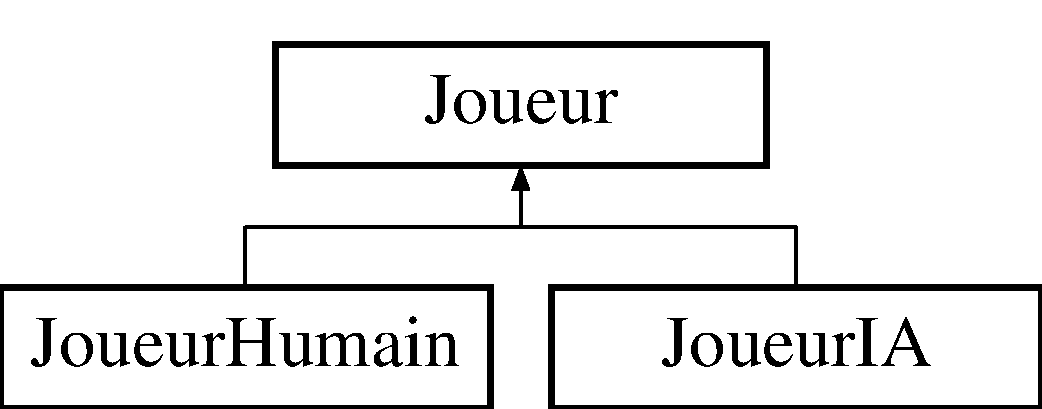
\includegraphics[height=2.000000cm]{class_joueur}
\end{center}
\end{figure}
\subsection*{Fonctions membres publiques}
\begin{DoxyCompactItemize}
\item 
\hyperlink{class_joueur_a951f6cb508b2d681eac4be586b8aac5f}{Joueur} ()\hypertarget{class_joueur_a951f6cb508b2d681eac4be586b8aac5f}{}\label{class_joueur_a951f6cb508b2d681eac4be586b8aac5f}

\begin{DoxyCompactList}\small\item\em Constructeur de la classe \hyperlink{class_joueur}{Joueur} qui met ses caractéristiques en ses valeurs par défaut. \end{DoxyCompactList}\item 
virtual bool \hyperlink{class_joueur_aee337662730df358b20474cac70d83e6}{est\+Une\+IA} ()
\begin{DoxyCompactList}\small\item\em Permet de savoir si ce joueur est une IA. Est utile lorsque l\textquotesingle{}on manipule un \hyperlink{class_joueur}{Joueur} et que l\textquotesingle{}on ne sait pas s\textquotesingle{}il est IA ou Humain. \end{DoxyCompactList}\item 
void \hyperlink{class_joueur_a07c1eba4f8531d594380fbcaaab240f6}{reset\+Grilles} ()\hypertarget{class_joueur_a07c1eba4f8531d594380fbcaaab240f6}{}\label{class_joueur_a07c1eba4f8531d594380fbcaaab240f6}

\begin{DoxyCompactList}\small\item\em fonction qui alloue la mémoire pour la grille et la grille des tentatives et les remplie de 0, donc d\textquotesingle{}eau \end{DoxyCompactList}\item 
void \hyperlink{class_joueur_a1f4357df61efbc2ead45d24a190ebb83}{definir\+Bateaux\+Type2} (int nb\+Max\+De\+Bateaux, int taille\+Grille)
\begin{DoxyCompactList}\small\item\em function permettant de définir un tableau de bateaux de tailles aléatoires \end{DoxyCompactList}\item 
void \hyperlink{class_joueur_a7f016748c27a4ddad2d363f4b5121ab1}{set\+Nom} (std\+::string nouveau\+Nom)
\begin{DoxyCompactList}\small\item\em fonction qui modifie l\textquotesingle{}attribut nom \end{DoxyCompactList}\item 
void \hyperlink{class_joueur_a424aec3294ea6019f372fd2d67ae5001}{set\+Grille} (char $\ast$$\ast$\hyperlink{class_joueur_a97a052f0b9966c94c49862df3144a62f}{grille}, int h, int l)
\begin{DoxyCompactList}\small\item\em fonction qui modifie les caractéristiques de la grille \end{DoxyCompactList}\item 
void \hyperlink{class_joueur_a11942778d97fd6f5823d8ef1ab964047}{set\+Grille\+Tentatives} (char $\ast$$\ast$\hyperlink{class_joueur_abbef5ee9c9c05a24ffa2c462e14cdfd7}{grille\+Tentatives})
\begin{DoxyCompactList}\small\item\em fonction qui modifie l\textquotesingle{}attribut grille\+Tentatives \end{DoxyCompactList}\item 
virtual void \hyperlink{class_joueur_a9027bfc622d9a175340b5fffe915c7b2}{demander\+Nom} ()\hypertarget{class_joueur_a9027bfc622d9a175340b5fffe915c7b2}{}\label{class_joueur_a9027bfc622d9a175340b5fffe915c7b2}

\begin{DoxyCompactList}\small\item\em initialise le nom du joueur en demandant le nom au joueur \end{DoxyCompactList}\item 
virtual void \hyperlink{class_joueur_a58fe79e4845404f361d5bc0fe9474135}{demander\+Taille\+Grille} ()\hypertarget{class_joueur_a58fe79e4845404f361d5bc0fe9474135}{}\label{class_joueur_a58fe79e4845404f361d5bc0fe9474135}

\begin{DoxyCompactList}\small\item\em initialise la taille de la grille en la demandant au joueur \end{DoxyCompactList}\item 
virtual char \hyperlink{class_joueur_a72fcb63683baba74922df5de246bff6f}{demander\+Type\+Jeu} ()\hypertarget{class_joueur_a72fcb63683baba74922df5de246bff6f}{}\label{class_joueur_a72fcb63683baba74922df5de246bff6f}

\begin{DoxyCompactList}\small\item\em fonction qui permet au joueur de choisir son type de jeu \+: bataille classique ou bataille améliorée \end{DoxyCompactList}\item 
virtual void \hyperlink{class_joueur_a5f0ab55bcb47e6808e46ef4515ce9565}{placement\+Des\+Bateaux} (char type\+Jeu)
\begin{DoxyCompactList}\small\item\em demande au joueur de placer ses différents bateaux. Utilise ajout\+Bateau pour chaqun des bateaux du joueur. \end{DoxyCompactList}\item 
virtual int $\ast$ \hyperlink{class_joueur_a46bdd92b73a1f0d04aeb5f19f33720b0}{tour} ()
\begin{DoxyCompactList}\small\item\em Permet de placer une bombe, affiche aussi la grille et la grille de tentatives. \end{DoxyCompactList}\item 
virtual void \hyperlink{class_joueur_a661426005c03ad2ee421249758f5c2a7}{resultat\+Bombe} (bool touche, int x, int y)
\begin{DoxyCompactList}\small\item\em Notifie le joueur si sa bombe a touché l\textquotesingle{}adversaire. \end{DoxyCompactList}\item 
virtual void \hyperlink{class_joueur_aeb9de0a7501a5370d45e670e122b3676}{resultat\+Bombe\+Adverse} (bool touche, int x, int y)
\begin{DoxyCompactList}\small\item\em Notifie le joueur si la bombe de l\textquotesingle{}adversaire l\textquotesingle{}a touché. \end{DoxyCompactList}\end{DoxyCompactItemize}
\subsection*{Fonctions membres protégées}
\begin{DoxyCompactItemize}
\item 
virtual void \hyperlink{class_joueur_a817129cc5062c058a153a241c74eee79}{placer\+Bateau} (\hyperlink{class_bateau}{Bateau} $\ast$b)
\begin{DoxyCompactList}\small\item\em Permet au joueur de positionner le bateau {\ttfamily $\ast$b} sur la grille. Cette fonction lui demande les coordonnées en x, y du bateau (en utilisant la fonction demander\+Coordonnees\+Bateau) mais aussi son orientation. \end{DoxyCompactList}\item 
void \hyperlink{class_joueur_ab42cd00f0ff47934eecde3fbaf06f2a5}{marquer\+Resultat\+Bombe\+Sur\+Grille\+Tentative} (bool touche, int x, int y)
\begin{DoxyCompactList}\small\item\em function permettant de modifier une case de la grille des tentatives sachant les conséquences de la bombe \end{DoxyCompactList}\item 
void \hyperlink{class_joueur_a3b77de3d2a5d2845bfefddb051460e80}{marquer\+Resultat\+Bombe\+Sur\+Grille} (bool touche, int x, int y)
\begin{DoxyCompactList}\small\item\em function permettant de modifier une case de la grille sachant les conséquences de la bombe \end{DoxyCompactList}\end{DoxyCompactItemize}
\subsection*{Attributs protégés}
\begin{DoxyCompactItemize}
\item 
std\+::string \hyperlink{class_joueur_abaee0b4f259181bf66dbab54bef971bb}{nom}
\item 
\hyperlink{class_grille}{Grille} \hyperlink{class_joueur_a97a052f0b9966c94c49862df3144a62f}{grille}
\item 
\hyperlink{class_grille}{Grille} \hyperlink{class_joueur_abbef5ee9c9c05a24ffa2c462e14cdfd7}{grille\+Tentatives}
\item 
int \hyperlink{class_joueur_a3a41069191547937ddd3acd15eecd4ee}{nb\+Cases\+Bateaux\+Touches}
\item 
int \hyperlink{class_joueur_a29e4485fe7b0a3f2c962757b7c7bf2a5}{nb\+Cases\+Bateaux}
\item 
int \hyperlink{class_joueur_a56752b0a96da94b17b07fd0312035a13}{nb\+Bateaux}
\item 
\hyperlink{class_bateau}{Bateau} $\ast$ \hyperlink{class_joueur_acf537ce482b493555318da7da14d8ac9}{bateaux}
\item 
\hyperlink{class_affichage}{Affichage} $\ast$ \hyperlink{class_joueur_a388634e5c242146dad447bc04756bab5}{affichage}
\end{DoxyCompactItemize}
\subsection*{Amis}
\begin{DoxyCompactItemize}
\item 
class {\bfseries Jeu\+Bataille\+Navale}\hypertarget{class_joueur_a5e820295bb9a9381c14f9067e97ca6c1}{}\label{class_joueur_a5e820295bb9a9381c14f9067e97ca6c1}

\end{DoxyCompactItemize}


\subsection{Description détaillée}
classe \hyperlink{class_joueur}{Joueur} regroupant les fonctionnalités générales sur le joueur 

\subsection{Documentation des fonctions membres}
\index{Joueur@{Joueur}!definir\+Bateaux\+Type2@{definir\+Bateaux\+Type2}}
\index{definir\+Bateaux\+Type2@{definir\+Bateaux\+Type2}!Joueur@{Joueur}}
\subsubsection[{\texorpdfstring{definir\+Bateaux\+Type2(int nb\+Max\+De\+Bateaux, int taille\+Grille)}{definirBateauxType2(int nbMaxDeBateaux, int tailleGrille)}}]{\setlength{\rightskip}{0pt plus 5cm}public Joueur\+::definir\+Bateaux\+Type2 (
\begin{DoxyParamCaption}
\item[{int}]{nb\+Max\+De\+Bateaux, }
\item[{int}]{taille\+Grille}
\end{DoxyParamCaption}
)}\hypertarget{class_joueur_a1f4357df61efbc2ead45d24a190ebb83}{}\label{class_joueur_a1f4357df61efbc2ead45d24a190ebb83}


function permettant de définir un tableau de bateaux de tailles aléatoires 


\begin{DoxyParams}{Paramètres}
{\em nb\+Max\+De\+Bateaux,taille\+Grille} & le nombre de bateaux du tableau et la taille de la grille \\
\hline
\end{DoxyParams}
\index{Joueur@{Joueur}!est\+Une\+IA@{est\+Une\+IA}}
\index{est\+Une\+IA@{est\+Une\+IA}!Joueur@{Joueur}}
\subsubsection[{\texorpdfstring{est\+Une\+I\+A()}{estUneIA()}}]{\setlength{\rightskip}{0pt plus 5cm}public Joueur\+::est\+Une\+IA (
\begin{DoxyParamCaption}
{}
\end{DoxyParamCaption}
)\hspace{0.3cm}{\ttfamily [inline]}, {\ttfamily [virtual]}}\hypertarget{class_joueur_aee337662730df358b20474cac70d83e6}{}\label{class_joueur_aee337662730df358b20474cac70d83e6}


Permet de savoir si ce joueur est une IA. Est utile lorsque l\textquotesingle{}on manipule un \hyperlink{class_joueur}{Joueur} et que l\textquotesingle{}on ne sait pas s\textquotesingle{}il est IA ou Humain. 

\begin{DoxyReturn}{Renvoie}
true si c\textquotesingle{}est une IA, false sinon. 
\end{DoxyReturn}


Réimplémentée dans \hyperlink{class_joueur_i_a_a549e94b2b4673dcf97041add34bc49a0}{Joueur\+IA}, et \hyperlink{class_joueur_humain_a4d531faca2e5f81966ff11309bd1fd9e}{Joueur\+Humain}.

\index{Joueur@{Joueur}!marquer\+Resultat\+Bombe\+Sur\+Grille@{marquer\+Resultat\+Bombe\+Sur\+Grille}}
\index{marquer\+Resultat\+Bombe\+Sur\+Grille@{marquer\+Resultat\+Bombe\+Sur\+Grille}!Joueur@{Joueur}}
\subsubsection[{\texorpdfstring{marquer\+Resultat\+Bombe\+Sur\+Grille(bool touche, int x, int y)}{marquerResultatBombeSurGrille(bool touche, int x, int y)}}]{\setlength{\rightskip}{0pt plus 5cm}protected Joueur\+::marquer\+Resultat\+Bombe\+Sur\+Grille (
\begin{DoxyParamCaption}
\item[{bool}]{touche, }
\item[{int}]{x, }
\item[{int}]{y}
\end{DoxyParamCaption}
)\hspace{0.3cm}{\ttfamily [protected]}}\hypertarget{class_joueur_a3b77de3d2a5d2845bfefddb051460e80}{}\label{class_joueur_a3b77de3d2a5d2845bfefddb051460e80}


function permettant de modifier une case de la grille sachant les conséquences de la bombe 


\begin{DoxyParams}{Paramètres}
{\em touche,x,y} & les coordonnées de la position à modifier, et touche\+: l\textquotesingle{}indication si la bombe a atteint sa cible \\
\hline
\end{DoxyParams}
\index{Joueur@{Joueur}!marquer\+Resultat\+Bombe\+Sur\+Grille\+Tentative@{marquer\+Resultat\+Bombe\+Sur\+Grille\+Tentative}}
\index{marquer\+Resultat\+Bombe\+Sur\+Grille\+Tentative@{marquer\+Resultat\+Bombe\+Sur\+Grille\+Tentative}!Joueur@{Joueur}}
\subsubsection[{\texorpdfstring{marquer\+Resultat\+Bombe\+Sur\+Grille\+Tentative(bool touche, int x, int y)}{marquerResultatBombeSurGrilleTentative(bool touche, int x, int y)}}]{\setlength{\rightskip}{0pt plus 5cm}protected Joueur\+::marquer\+Resultat\+Bombe\+Sur\+Grille\+Tentative (
\begin{DoxyParamCaption}
\item[{bool}]{touche, }
\item[{int}]{x, }
\item[{int}]{y}
\end{DoxyParamCaption}
)\hspace{0.3cm}{\ttfamily [protected]}}\hypertarget{class_joueur_ab42cd00f0ff47934eecde3fbaf06f2a5}{}\label{class_joueur_ab42cd00f0ff47934eecde3fbaf06f2a5}


function permettant de modifier une case de la grille des tentatives sachant les conséquences de la bombe 


\begin{DoxyParams}{Paramètres}
{\em touche,x,y} & les coordonnées de la position à modifier, et touche\+: l\textquotesingle{}indication si la bombe a atteint sa cible \\
\hline
\end{DoxyParams}
\index{Joueur@{Joueur}!placement\+Des\+Bateaux@{placement\+Des\+Bateaux}}
\index{placement\+Des\+Bateaux@{placement\+Des\+Bateaux}!Joueur@{Joueur}}
\subsubsection[{\texorpdfstring{placement\+Des\+Bateaux(char type\+Jeu)}{placementDesBateaux(char typeJeu)}}]{\setlength{\rightskip}{0pt plus 5cm}public Joueur\+::placement\+Des\+Bateaux (
\begin{DoxyParamCaption}
\item[{char}]{type\+Jeu}
\end{DoxyParamCaption}
)\hspace{0.3cm}{\ttfamily [inline]}, {\ttfamily [virtual]}}\hypertarget{class_joueur_a5f0ab55bcb47e6808e46ef4515ce9565}{}\label{class_joueur_a5f0ab55bcb47e6808e46ef4515ce9565}


demande au joueur de placer ses différents bateaux. Utilise ajout\+Bateau pour chaqun des bateaux du joueur. 


\begin{DoxyParams}{Paramètres}
{\em type\+Jeu} & le type de jeu choisis \\
\hline
\end{DoxyParams}


Réimplémentée dans \hyperlink{class_joueur_i_a_a6d7592fa8c653cb5420270d61467419b}{Joueur\+IA}, et \hyperlink{class_joueur_humain_ae27bf69ba0db87cd8268ba1cd1e4f817}{Joueur\+Humain}.

\index{Joueur@{Joueur}!placer\+Bateau@{placer\+Bateau}}
\index{placer\+Bateau@{placer\+Bateau}!Joueur@{Joueur}}
\subsubsection[{\texorpdfstring{placer\+Bateau(\+Bateau $\ast$b)}{placerBateau(Bateau *b)}}]{\setlength{\rightskip}{0pt plus 5cm}protected Joueur\+::placer\+Bateau (
\begin{DoxyParamCaption}
\item[{{\bf Bateau} $\ast$}]{b}
\end{DoxyParamCaption}
)\hspace{0.3cm}{\ttfamily [inline]}, {\ttfamily [protected]}, {\ttfamily [virtual]}}\hypertarget{class_joueur_a817129cc5062c058a153a241c74eee79}{}\label{class_joueur_a817129cc5062c058a153a241c74eee79}


Permet au joueur de positionner le bateau {\ttfamily $\ast$b} sur la grille. Cette fonction lui demande les coordonnées en x, y du bateau (en utilisant la fonction demander\+Coordonnees\+Bateau) mais aussi son orientation. 


\begin{DoxyParams}{Paramètres}
{\em $\ast$b} & Un pointeur sur le bateau que le joueur va placer sur la grille. \\
\hline
\end{DoxyParams}


Réimplémentée dans \hyperlink{class_joueur_humain_af9e3ccafc7cde958dda81551d0ef6abd}{Joueur\+Humain}, et \hyperlink{class_joueur_i_a_a70a56322ca6eeeb52612510d7e22d388}{Joueur\+IA}.

\index{Joueur@{Joueur}!resultat\+Bombe@{resultat\+Bombe}}
\index{resultat\+Bombe@{resultat\+Bombe}!Joueur@{Joueur}}
\subsubsection[{\texorpdfstring{resultat\+Bombe(bool touche, int x, int y)}{resultatBombe(bool touche, int x, int y)}}]{\setlength{\rightskip}{0pt plus 5cm}public Joueur\+::resultat\+Bombe (
\begin{DoxyParamCaption}
\item[{bool}]{touche, }
\item[{int}]{x, }
\item[{int}]{y}
\end{DoxyParamCaption}
)\hspace{0.3cm}{\ttfamily [inline]}, {\ttfamily [virtual]}}\hypertarget{class_joueur_a661426005c03ad2ee421249758f5c2a7}{}\label{class_joueur_a661426005c03ad2ee421249758f5c2a7}


Notifie le joueur si sa bombe a touché l\textquotesingle{}adversaire. 


\begin{DoxyParams}{Paramètres}
{\em touche} & true si la bombe a touché un navire adverse, false sinon. \\
\hline
{\em x} & La coordonnée en x de la bombe que le joueur avait choisie. \\
\hline
{\em y} & La coordonnée en y de la bombe que le joueur avait choisie. \\
\hline
\end{DoxyParams}


Réimplémentée dans \hyperlink{class_joueur_i_a_a5e7ed6369200fe44382a54cf739ad8b3}{Joueur\+IA}, et \hyperlink{class_joueur_humain_a9eeae3b54b174e477a94c75d57a0d403}{Joueur\+Humain}.

\index{Joueur@{Joueur}!resultat\+Bombe\+Adverse@{resultat\+Bombe\+Adverse}}
\index{resultat\+Bombe\+Adverse@{resultat\+Bombe\+Adverse}!Joueur@{Joueur}}
\subsubsection[{\texorpdfstring{resultat\+Bombe\+Adverse(bool touche, int x, int y)}{resultatBombeAdverse(bool touche, int x, int y)}}]{\setlength{\rightskip}{0pt plus 5cm}public Joueur\+::resultat\+Bombe\+Adverse (
\begin{DoxyParamCaption}
\item[{bool}]{touche, }
\item[{int}]{x, }
\item[{int}]{y}
\end{DoxyParamCaption}
)\hspace{0.3cm}{\ttfamily [inline]}, {\ttfamily [virtual]}}\hypertarget{class_joueur_aeb9de0a7501a5370d45e670e122b3676}{}\label{class_joueur_aeb9de0a7501a5370d45e670e122b3676}


Notifie le joueur si la bombe de l\textquotesingle{}adversaire l\textquotesingle{}a touché. 


\begin{DoxyParams}{Paramètres}
{\em touche} & true si la bombe a touché un navire, false sinon. \\
\hline
{\em x} & La coordonnée en x de la bombe que le joueur adverse avait choisie. \\
\hline
{\em y} & La coordonnée en y de la bombe que le joueur adverse avait choisie. \\
\hline
\end{DoxyParams}


Réimplémentée dans \hyperlink{class_joueur_i_a_a35dfe27baa0fb62a927cc13186b09920}{Joueur\+IA}, et \hyperlink{class_joueur_humain_acdd6b332153e1543d083d272fbdf8289}{Joueur\+Humain}.

\index{Joueur@{Joueur}!set\+Grille@{set\+Grille}}
\index{set\+Grille@{set\+Grille}!Joueur@{Joueur}}
\subsubsection[{\texorpdfstring{set\+Grille(char $\ast$$\ast$grille, int h, int l)}{setGrille(char **grille, int h, int l)}}]{\setlength{\rightskip}{0pt plus 5cm}public Joueur\+::set\+Grille (
\begin{DoxyParamCaption}
\item[{char $\ast$$\ast$}]{grille, }
\item[{int}]{h, }
\item[{int}]{l}
\end{DoxyParamCaption}
)}\hypertarget{class_joueur_a424aec3294ea6019f372fd2d67ae5001}{}\label{class_joueur_a424aec3294ea6019f372fd2d67ae5001}


fonction qui modifie les caractéristiques de la grille 


\begin{DoxyParams}{Paramètres}
{\em grille,h,l} & grille\+: object modifié, hauteur, largueur \\
\hline
\end{DoxyParams}
\index{Joueur@{Joueur}!set\+Grille\+Tentatives@{set\+Grille\+Tentatives}}
\index{set\+Grille\+Tentatives@{set\+Grille\+Tentatives}!Joueur@{Joueur}}
\subsubsection[{\texorpdfstring{set\+Grille\+Tentatives(char $\ast$$\ast$grille\+Tentatives)}{setGrilleTentatives(char **grilleTentatives)}}]{\setlength{\rightskip}{0pt plus 5cm}public Joueur\+::set\+Grille\+Tentatives (
\begin{DoxyParamCaption}
\item[{char $\ast$$\ast$}]{grille\+Tentatives}
\end{DoxyParamCaption}
)}\hypertarget{class_joueur_a11942778d97fd6f5823d8ef1ab964047}{}\label{class_joueur_a11942778d97fd6f5823d8ef1ab964047}


fonction qui modifie l\textquotesingle{}attribut grille\+Tentatives 


\begin{DoxyParams}{Paramètres}
{\em $\ast$$\ast$grille\+Tentatives} & \\
\hline
\end{DoxyParams}
\index{Joueur@{Joueur}!set\+Nom@{set\+Nom}}
\index{set\+Nom@{set\+Nom}!Joueur@{Joueur}}
\subsubsection[{\texorpdfstring{set\+Nom(std\+::string nouveau\+Nom)}{setNom(std::string nouveauNom)}}]{\setlength{\rightskip}{0pt plus 5cm}public Joueur\+::set\+Nom (
\begin{DoxyParamCaption}
\item[{std\+::string}]{nouveau\+Nom}
\end{DoxyParamCaption}
)}\hypertarget{class_joueur_a7f016748c27a4ddad2d363f4b5121ab1}{}\label{class_joueur_a7f016748c27a4ddad2d363f4b5121ab1}


fonction qui modifie l\textquotesingle{}attribut nom 


\begin{DoxyParams}{Paramètres}
{\em nouveau\+Nom} & \\
\hline
\end{DoxyParams}
\index{Joueur@{Joueur}!tour@{tour}}
\index{tour@{tour}!Joueur@{Joueur}}
\subsubsection[{\texorpdfstring{tour()}{tour()}}]{\setlength{\rightskip}{0pt plus 5cm}public Joueur\+::tour (
\begin{DoxyParamCaption}
{}
\end{DoxyParamCaption}
)\hspace{0.3cm}{\ttfamily [inline]}, {\ttfamily [virtual]}}\hypertarget{class_joueur_a46bdd92b73a1f0d04aeb5f19f33720b0}{}\label{class_joueur_a46bdd92b73a1f0d04aeb5f19f33720b0}


Permet de placer une bombe, affiche aussi la grille et la grille de tentatives. 

\begin{DoxyReturn}{Renvoie}
Les coordonnées de la bombe cible. Sous la forme d\textquotesingle{}un tableau \mbox{[}x, y\mbox{]}. 
\end{DoxyReturn}


Réimplémentée dans \hyperlink{class_joueur_i_a_a76b3e9af59c86acb34d7e1cb70802436}{Joueur\+IA}, et \hyperlink{class_joueur_humain_a92f4cb99ff2957813da34fb60e211870}{Joueur\+Humain}.



\subsection{Documentation des données membres}
\index{Joueur@{Joueur}!affichage@{affichage}}
\index{affichage@{affichage}!Joueur@{Joueur}}
\subsubsection[{\texorpdfstring{affichage}{affichage}}]{\setlength{\rightskip}{0pt plus 5cm}{\bf Affichage}$\ast$ Joueur\+::affichage\hspace{0.3cm}{\ttfamily [protected]}}\hypertarget{class_joueur_a388634e5c242146dad447bc04756bab5}{}\label{class_joueur_a388634e5c242146dad447bc04756bab5}
Un affichage pour afficher des informations générales sur le jeux. \index{Joueur@{Joueur}!bateaux@{bateaux}}
\index{bateaux@{bateaux}!Joueur@{Joueur}}
\subsubsection[{\texorpdfstring{bateaux}{bateaux}}]{\setlength{\rightskip}{0pt plus 5cm}{\bf Bateau}$\ast$ Joueur\+::bateaux\hspace{0.3cm}{\ttfamily [protected]}}\hypertarget{class_joueur_acf537ce482b493555318da7da14d8ac9}{}\label{class_joueur_acf537ce482b493555318da7da14d8ac9}
Un tableau contenant les bateaux possédés par le joueur et qu\textquotesingle{}il a placé sur la grille. \index{Joueur@{Joueur}!grille@{grille}}
\index{grille@{grille}!Joueur@{Joueur}}
\subsubsection[{\texorpdfstring{grille}{grille}}]{\setlength{\rightskip}{0pt plus 5cm}{\bf Grille} Joueur\+::grille\hspace{0.3cm}{\ttfamily [protected]}}\hypertarget{class_joueur_a97a052f0b9966c94c49862df3144a62f}{}\label{class_joueur_a97a052f0b9966c94c49862df3144a62f}
La grille sur laquelle le joueur place ses bateaux \index{Joueur@{Joueur}!grille\+Tentatives@{grille\+Tentatives}}
\index{grille\+Tentatives@{grille\+Tentatives}!Joueur@{Joueur}}
\subsubsection[{\texorpdfstring{grille\+Tentatives}{grilleTentatives}}]{\setlength{\rightskip}{0pt plus 5cm}{\bf Grille} Joueur\+::grille\+Tentatives\hspace{0.3cm}{\ttfamily [protected]}}\hypertarget{class_joueur_abbef5ee9c9c05a24ffa2c462e14cdfd7}{}\label{class_joueur_abbef5ee9c9c05a24ffa2c462e14cdfd7}
La grille permettant de garder en mémoire les tentatives de bombes effectuées par le joueur \index{Joueur@{Joueur}!nb\+Bateaux@{nb\+Bateaux}}
\index{nb\+Bateaux@{nb\+Bateaux}!Joueur@{Joueur}}
\subsubsection[{\texorpdfstring{nb\+Bateaux}{nbBateaux}}]{\setlength{\rightskip}{0pt plus 5cm}int Joueur\+::nb\+Bateaux\hspace{0.3cm}{\ttfamily [protected]}}\hypertarget{class_joueur_a56752b0a96da94b17b07fd0312035a13}{}\label{class_joueur_a56752b0a96da94b17b07fd0312035a13}
/ Le nombre de bateau initial du joueur. Permet de simplifier l\textquotesingle{}écriture de certaines boucles. ( i $<$ nb\+Bateaux etc) \index{Joueur@{Joueur}!nb\+Cases\+Bateaux@{nb\+Cases\+Bateaux}}
\index{nb\+Cases\+Bateaux@{nb\+Cases\+Bateaux}!Joueur@{Joueur}}
\subsubsection[{\texorpdfstring{nb\+Cases\+Bateaux}{nbCasesBateaux}}]{\setlength{\rightskip}{0pt plus 5cm}int Joueur\+::nb\+Cases\+Bateaux\hspace{0.3cm}{\ttfamily [protected]}}\hypertarget{class_joueur_a29e4485fe7b0a3f2c962757b7c7bf2a5}{}\label{class_joueur_a29e4485fe7b0a3f2c962757b7c7bf2a5}
Le nombre de cases occupées par des bateaux sur la grille \index{Joueur@{Joueur}!nb\+Cases\+Bateaux\+Touches@{nb\+Cases\+Bateaux\+Touches}}
\index{nb\+Cases\+Bateaux\+Touches@{nb\+Cases\+Bateaux\+Touches}!Joueur@{Joueur}}
\subsubsection[{\texorpdfstring{nb\+Cases\+Bateaux\+Touches}{nbCasesBateauxTouches}}]{\setlength{\rightskip}{0pt plus 5cm}int Joueur\+::nb\+Cases\+Bateaux\+Touches\hspace{0.3cm}{\ttfamily [protected]}}\hypertarget{class_joueur_a3a41069191547937ddd3acd15eecd4ee}{}\label{class_joueur_a3a41069191547937ddd3acd15eecd4ee}
Correspond au nombre de fois que l\textquotesingle{}adversaire a touché un bateau.\+Va être incrementé quand un des bateaux est touché pour faciliter la vérification de la fin de partie. \index{Joueur@{Joueur}!nom@{nom}}
\index{nom@{nom}!Joueur@{Joueur}}
\subsubsection[{\texorpdfstring{nom}{nom}}]{\setlength{\rightskip}{0pt plus 5cm}std\+::string Joueur\+::nom\hspace{0.3cm}{\ttfamily [protected]}}\hypertarget{class_joueur_abaee0b4f259181bf66dbab54bef971bb}{}\label{class_joueur_abaee0b4f259181bf66dbab54bef971bb}
Le nom du joueur 

La documentation de cette classe a été générée à partir des fichiers suivants \+:\begin{DoxyCompactItemize}
\item 
/home/lucas/\+Documents/\+Git\+Hub/\+Bataille-\/\+Navale/src/\hyperlink{_joueur_8hpp}{Joueur.\+hpp}\item 
/home/lucas/\+Documents/\+Git\+Hub/\+Bataille-\/\+Navale/src/Joueur.\+cpp\end{DoxyCompactItemize}

\chapter{Documentation des fichiers}
\hypertarget{_bateau_8hpp}{}\section{Référence du fichier /home/lucas/\+Documents/\+Git\+Hub/\+Bataille-\/\+Navale/src/\+Bateau.hpp}
\label{_bateau_8hpp}\index{/home/lucas/\+Documents/\+Git\+Hub/\+Bataille-\/\+Navale/src/\+Bateau.\+hpp@{/home/lucas/\+Documents/\+Git\+Hub/\+Bataille-\/\+Navale/src/\+Bateau.\+hpp}}


classe \hyperlink{class_bateau}{Bateau}  


{\ttfamily \#include \char`\"{}Grille.\+hpp\char`\"{}}\\*
\subsection*{Classes}
\begin{DoxyCompactItemize}
\item 
class \hyperlink{class_bateau}{Bateau}
\begin{DoxyCompactList}\small\item\em classe fixant des bateaux au début de la partie. L\textquotesingle{}extrémité d\textquotesingle{}un bateau est située en haut et à gauche. C\textquotesingle{}est à dire que l\textquotesingle{}éxtrémité d\textquotesingle{}un bateau situé en position verticale est en haut et l\textquotesingle{}éxtrémité d\textquotesingle{}un bateau situé à l\textquotesingle{}horizontale est à gauche. \end{DoxyCompactList}\end{DoxyCompactItemize}


\subsection{Description détaillée}
classe \hyperlink{class_bateau}{Bateau} 

\begin{DoxyAuthor}{Auteur}
Groupe B7 
\end{DoxyAuthor}
\begin{DoxyVersion}{Version}
0.\+1 
\end{DoxyVersion}
\begin{DoxyDate}{Date}
22 mai 2018 Classe \hyperlink{class_bateau}{Bateau} qui fixe des bateaux au début de la partie 
\end{DoxyDate}

\hypertarget{_grille_8hpp}{}\section{Référence du fichier D\+:/\+Documents/\+Git\+Hub/\+Bataille-\/\+Navale/src/\+Grille.hpp}
\label{_grille_8hpp}\index{D\+:/\+Documents/\+Git\+Hub/\+Bataille-\/\+Navale/src/\+Grille.\+hpp@{D\+:/\+Documents/\+Git\+Hub/\+Bataille-\/\+Navale/src/\+Grille.\+hpp}}


classe \mbox{\hyperlink{class_grille}{Grille}}  


{\ttfamily \#include \char`\"{}Bateau.\+hpp\char`\"{}}\newline
\subsection*{Classes}
\begin{DoxyCompactItemize}
\item 
class \mbox{\hyperlink{class_grille}{Grille}}
\end{DoxyCompactItemize}


\subsection{Description détaillée}
classe \mbox{\hyperlink{class_grille}{Grille}} 

\begin{DoxyAuthor}{Auteur}
Groupe B7 
\end{DoxyAuthor}
\begin{DoxyVersion}{Version}
0.\+1 
\end{DoxyVersion}
\begin{DoxyDate}{Date}
13 avril 2018 Classe \mbox{\hyperlink{class_grille}{Grille}} qui gère la modification et l\textquotesingle{}affichage de la grille 
\end{DoxyDate}

\hypertarget{_jeu_bataille_navale_8hpp}{}\section{Référence du fichier /home/lucas/\+Documents/\+Git\+Hub/\+Bataille-\/\+Navale/src/\+Jeu\+Bataille\+Navale.hpp}
\label{_jeu_bataille_navale_8hpp}\index{/home/lucas/\+Documents/\+Git\+Hub/\+Bataille-\/\+Navale/src/\+Jeu\+Bataille\+Navale.\+hpp@{/home/lucas/\+Documents/\+Git\+Hub/\+Bataille-\/\+Navale/src/\+Jeu\+Bataille\+Navale.\+hpp}}


classe \hyperlink{class_jeu_bataille_navale}{Jeu\+Bataille\+Navale}  


{\ttfamily \#include \char`\"{}Affichage.\+hpp\char`\"{}}\\*
{\ttfamily \#include \char`\"{}Joueur.\+hpp\char`\"{}}\\*
{\ttfamily \#include \char`\"{}Joueur\+Humain.\+hpp\char`\"{}}\\*
{\ttfamily \#include \char`\"{}Joueur\+I\+A.\+hpp\char`\"{}}\\*
{\ttfamily \#include \char`\"{}Gestion\+Sauvegarde.\+hpp\char`\"{}}\\*
\subsection*{Classes}
\begin{DoxyCompactItemize}
\item 
class \hyperlink{class_jeu_bataille_navale}{Jeu\+Bataille\+Navale}
\begin{DoxyCompactList}\small\item\em classe qui gère le déroulement du jeu de Bataille Navale. \end{DoxyCompactList}\end{DoxyCompactItemize}


\subsection{Description détaillée}
classe \hyperlink{class_jeu_bataille_navale}{Jeu\+Bataille\+Navale} 

\begin{DoxyAuthor}{Auteur}
groupe B7 
\end{DoxyAuthor}
\begin{DoxyVersion}{Version}
0.\+1 
\end{DoxyVersion}
\begin{DoxyDate}{Date}
22 mai 2018
\end{DoxyDate}
Classe \hyperlink{class_jeu_bataille_navale}{Jeu\+Bataille\+Navale}, classe principale qui contrôle la partie entre les deux joueurs. 
\hypertarget{_joueur_8hpp}{}\section{Joueur.\+hpp File Reference}
\label{_joueur_8hpp}\index{Joueur.\+hpp@{Joueur.\+hpp}}


classe \mbox{\hyperlink{class_jeu_bataille_navale}{Jeu\+Bataille\+Navale}}  


{\ttfamily \#include $<$string$>$}\newline
{\ttfamily \#include \char`\"{}Grille.\+hpp\char`\"{}}\newline
{\ttfamily \#include \char`\"{}Bateau.\+hpp\char`\"{}}\newline
\subsection*{Classes}
\begin{DoxyCompactItemize}
\item 
class \mbox{\hyperlink{class_joueur}{Joueur}}
\begin{DoxyCompactList}\small\item\em classe representant le joueur \end{DoxyCompactList}\end{DoxyCompactItemize}


\subsection{Detailed Description}
classe \mbox{\hyperlink{class_jeu_bataille_navale}{Jeu\+Bataille\+Navale}} 

\begin{DoxyAuthor}{Author}
groupe B7 
\end{DoxyAuthor}
\begin{DoxyVersion}{Version}
0.\+1 
\end{DoxyVersion}
\begin{DoxyDate}{Date}
13 Avril 2018
\end{DoxyDate}
Classe \mbox{\hyperlink{class_joueur}{Joueur}}, classe qui contrôle ce que peuvent faire les joueurs durant la partie. 
%--- End generated contents ---

% Index
\backmatter
\newpage
\phantomsection
\clearemptydoublepage
\addcontentsline{toc}{chapter}{Index}
\printindex

\end{document}
